\subsection{Loop antenna with gap}\label{sec:loop_gap_sim}
\subsubsection{Setup and geometrical analysis}
\FloatBarrier
\begin{figure}[h]
	\centering
	\includegraphics[width=0.5\linewidth]{content/img/gapped_loop_antenna}
	\caption{Geometry of loop antenna with a gap in the return path inserted in the TEM cell.}
	\label{fig:gappedloopantenna}
\end{figure}

The geometry of the loop antenna with a gap is similar to that of the loop antenna discussed in \autoref{sec:loop_sim}. A gap is present with $10\,\upmu\mathrm{m}$ height in the return path, as shown in \autoref{fig:gappedloopantenna}. The magnetic coupling is determined with \crefrange{eqn:e_a_closed_int}{eqn:e_b_closed_int}, leading to 

\begin{equation}
	-\oint_C \boldsymbol{\tau} I(l) \cdot\mathbf{e}_n^\pm  dl= -\int_\text{wire} \boldsymbol{\tau} I_\text{wire}(l) \cdot\mathbf{e}_n^\pm  dl -\int_\text{gap} \boldsymbol{\tau} I_\text{gap}(l) \cdot\mathbf{e}_n^\pm  dl.
\end{equation}

The electric current in the gap is $I_\mathrm{gap}=0\,\mathrm{A}$, while the current in the antenna wire $I_\mathrm{wire}$ is significantly reduced due to the interrupted current path. Consequently, the magnetic coupling between the loop antenna with a gap and the TEM cell is expected to be lower than that of the loop antenna without a gap.

The conductors around the gap act as capacitors, accumulating charges on both sides. This leads to a higher potential in the wire of the antenna. The electric coupling increases significantly, according to \crefrange{eqn:charges_a}{eqn:charges_b}. Concluding, the structure of the loop antenna with the gap suggests capacitive behavior with a dominating electric dipole moment.

\todo[inline]{TODO: Some sources state that electrically small antennas must be either strongly capacitive or inductive. This would mean, that small antennas can always be represented by the same model: Either dominating electric dipole moment in the capacitive antenna case, with a non-linear behavior of the high frequencies, or a magnetic dipole moment with the same property in the inductive antenna case. The frequency, at which the non-linearities occur, depend on the amount of capacitance or inductance, i.e. the Q-factor. A high Q-factor leads to non-linearities in lower cut-off frequencies, and a low Q-factor increases the cut-off frequency. A capacitive antenna with low impedance has a high Q-factor. A inductive antenna with high impedance has a high Q-factor. This can practically be read from the impedance graphs. Can a relation between the impedance/Q-factor and a ``cut-off frequency'' of the dipole moments be established?}

\todo[inline]{TODO: A little thought experiment on the gapped loop antenna demonstrates why this is the case: If the magnetic dipole moment shall be increased in this antenna, the height of the gap can be decreased to increase the current flow and therefore the magnetic coupling. Ironically, this also increases the amount of charges accumulating on the boundaries of the gap, therefore increasing the electric coupling and capacitive behavior. The capacitive behavior can therefore not change, unless the gap is completely removed. Also, the decrease in gap leads to larger total energy transfer and a higher Q-factor. I suspect, that a high Q-factor of an antenna leads to high energy transfer. This would make sense, because a high Q-factor indicates increased near-field intensities, that would naturally couple with the tem cell. A simulation showing the dipole moments for different gap heights over the frequency would support this claim.}

\FloatBarrier
\subsubsection{Equivalent dipole moments}
\FloatBarrier

The electric dipole moment shown in \autoref{fig:gappedloopmoments} clearly dominates over the magnetic dipole moment. The dipole moments behave non-linearly over the frequency. 

\begin{figure}[htbp]
	\centering
	\begin{subfigure}[t]{0.48\textwidth}
		\centering
		\includegraphics[width=1\linewidth]{content/img/gapped_loop_moments}
		\caption{}
		\label{fig:gappedloopmoments}
	\end{subfigure}
	\hfill
	\begin{subfigure}[t]{0.48\textwidth}
		\centering
		\includegraphics[width=1\linewidth]{content/img/gapped_loop_phase}
		\caption{}
		\label{fig:gappedloopphase}
	\end{subfigure}
	
	\caption{Dipole moments and phase shift of loop antenna}
	\label{fig:example}
\end{figure}

\autoref{fig:gappedloopcompmomentsgapsweep} demonstrates the effect of the gap height on the dipole moments' behavior. A larger gap height leads to an decreased charge concentration in the gap region, consequently a smaller magnitude of the electric dipole moment $\mathbf{m}_\mathrm{e}$. Additionally, it also leads to a decrease in electric current $\mathbf{J}$ in the antenna, reducing the magnetic dipole moment $\mathbf{m}_\mathrm{m}$. The reduction in the magnitude of $\mathbf{m}_\mathrm{e}$ and $\mathbf{m}_\mathrm{m}$ with increasing gap height is reflected in the decreasing output power shown in \autoref{fig:gappedloopcomppowergapsweep}.

\begin{figure}[htbp]
	\centering
	\begin{subfigure}[b]{0.48\textwidth}
		\centering
		\includegraphics[width=1\linewidth]{content/img/gapped_loop_comp_moments_gap_sweep}
		\caption{}
		\label{fig:gappedloopcompmomentsgapsweep}
	\end{subfigure}
	\hfill
	\begin{subfigure}[b]{0.48\textwidth}
		\centering
		\includegraphics[width=1\linewidth]{content/img/gapped_loop_comp_power_gap_sweep}
		\caption{}
		\label{fig:gappedloopcomppowergapsweep}
	\end{subfigure}
	
	\caption{Comparison of dipole moments and output power at different gap heights.}
	\label{fig:example}
\end{figure}

An increase in gap height reduces the non-linearities in $\mathbf{m}_\mathrm{e}$ and $\mathbf{m}_\mathrm{m}$. The voltage drop across the gap and the charge accumulation remains stabler over frequency. A small gap leads to both an increase in current and inductance, therefore creating a large voltage drop and influencing $\mathbf{m}_\mathrm{e}$ and $\mathbf{m}_\mathrm{m}$.

\FloatBarrier
\subsubsection{Electrical characteristics}
\FloatBarrier

\begin{figure}[htbp]
	\centering
	\begin{subfigure}[b]{0.48\textwidth}
		\centering
		\includegraphics[width=1\linewidth]{content/img/gapped_loop_opower}
		\caption{Output electric field and power}
		\label{fig:gappedloopopower}
	\end{subfigure}
	\hfill
	\begin{subfigure}[b]{0.48\textwidth}
		\centering
		\includegraphics[width=1\linewidth]{content/img/gapped_loop_voltage}
		\caption{Peak feed voltage}
		\label{fig:gappedloopvoltage}
	\end{subfigure}
	
	\caption{Electric field and power at the TEM cell's output port, and the peak feed voltage of the antenna.}
	\label{fig:example}
\end{figure}



\begin{figure}[htbp]
	\centering
	\begin{subfigure}[b]{0.48\textwidth}
		\centering
		\includegraphics[width=1\linewidth]{content/img/gapped_loop_current}
		\caption{RMS feed current.}
		\label{fig:gappedloopcurrent}
	\end{subfigure}
	\hfill
	\begin{subfigure}[b]{0.48\textwidth}
		\centering
		\includegraphics[width=1\linewidth]{content/img/gapped_loop_imp}
		\caption{Magnitude and phase of impedance}
		\label{fig:gappedloopimp}
	\end{subfigure}
	\label{fig:example}
\end{figure}

The inductance of this antenna is not negligible, opposed to the case of the monopole antenna in \autoref{sec:monopole}. This causes a significant magnitude of $\mathbf{m}_\mathrm{m}$ in \autoref{fig:gappedloopmoments} and a stronger decline in impedance magnitude of the loop antenna with gap, shown in \autoref{fig:gappedloopimp}, compared to the monopole antenna's impedance, demonstrated in \autoref{fig:monopoleimp}.



The gap leads to a significant reduction of electric current. Consequently, the impedance of the antenna shows capacitive behavior, as indicated in \autoref{fig:gappedloopim}. The energy transfer to the TEM cell occurs primarily by displacement current, explaining the dominating electric dipole moment due to \autoref{eqn:me_i}.

\FloatBarrier